\documentclass{article}
\usepackage{graphicx}
\DeclareGraphicsExtensions{.png}
\usepackage{hyperref}
\title{Code Theorie}
\date{2017-04-28}
\author{Siebert Aerts \and C\'{e}dric De Haes}

\begin{document}
	\section{VigenerePlus}
	\section{PlayFair}
	Het is ons niet gelukt om de PlayFair code te kraken.\\
	We probeerden dit te doen met behulp van de frequentie-analyse van bigrammen. Eerst hebben we een playfair decoder ge\"{i}mplemeteerd. Deze gaat een code nemen en die decoderen volgens een gegeven vierkant. Deze hebben we nodig omdat de tekst te klein is om brute force de frequentie te nemen van elk bigram in de code te vervangen door het bigram met ongeveer gelijke frequentie. Daarom maken we in de start een random vierkant aan als sleutel en decoderen we de code met behulp van deze decoder. Dan wordt op deze gedecodeerde tekst een score geplakt. Deze score wordt berekend aan de hand van de frequentie-analyse gevonden op \\ \url{https://fusiontables.google.com/DataSource?docid=15jK-3WUD-JjQMdwLe-ipwqkUdjvf2JKK-D-s9as}\\
	Vanuit die tabel worden de frequenties van alle bigrammen berekend. De dubbele letters worden in deze tabel worden eerlijk verdeeld over beide mogelijkheden met een X. De frequenties van bigrammen met een J worden opgeteld met die van overeenkomstige bigrammen met een I.\\
	De score wordt berekend door de som te nemen van de frequenties in de gedecodeerde tekst.
	Deze score wordt dat vergeleken met de score van enkele andere dichtbijzijnde sleutels:
	\begin{enumerate}
		\item 1 rij omhoog
		\item 1 rij omlaag
		\item 1 rij links
		\item 1 rij rechts
		\item 1 rij spiegelen
		\item 1 kolom spiegelen
		\item 2 random rijen omwisselen
		\item 2 random kolommen omwisselen
		\item een random pair karakters omwisselen
		\item 5 random pair karakters omwisselen
		\item 2 random pair karakters omwisselen
		\item een random triplet omwisselen
	\end{enumerate}
	Als de score van van al deze sleutels kleiner is dan die van de oorspronkelijke sleutel, is de oorspronkelijke sleutel de correcte sleutel. Dit wordt dan nog een aantal keren herhaald omdat je werkt met random waardes. Als er een sleutel wordt gevonden met een betere of gelijke score, dan worden dichtbijzijnde sleutels bij die sleutel gekozen.\\
	Op deze manier kwamen we relatief snel aan een oplossing, maar was deze steeds incorrect. Toen bedachten we ons dat de letters die niet in het codewoord staan in alfabetische volgorde achter het codewoord geplaatst worden om het vierkant op te vullen. Dus voegden we de voorwaarde toe dat de laatste 5 karakters van de sleutel in alfabetische volgorde moeten staan. Dit komt niet uit voor codewoorden met meer dan 20 verschillende letters (J niet meegerekend). Daarom dat we aannemen dat de sleutel toch correct is als in dezelfde sleutel 100 keer naar een betere sleutel gezocht werd.
	\section{ADFVGX}
	\section{Enigma}
	Het is ons ook niet gelukt om de enigma code te kraken.\\
	Eerst hebben we een Enigma machine ge\"{i}mplementeerd. Met behulp van de code en de crib maakten we intern een graaf aan de hand van een dictionary van lijsten. Omdat we geen makkelijk algoritme ken om alle onafhankelijke cycles in een graaf te vinden. Omdat de graaf relatief klein is (24 paden) hebben we die manueel getekent en de cycles op deze figuur aangeduid. Zo bekwamen we volgende graaf. 
	\begin{figure}[h!]
		\centering
		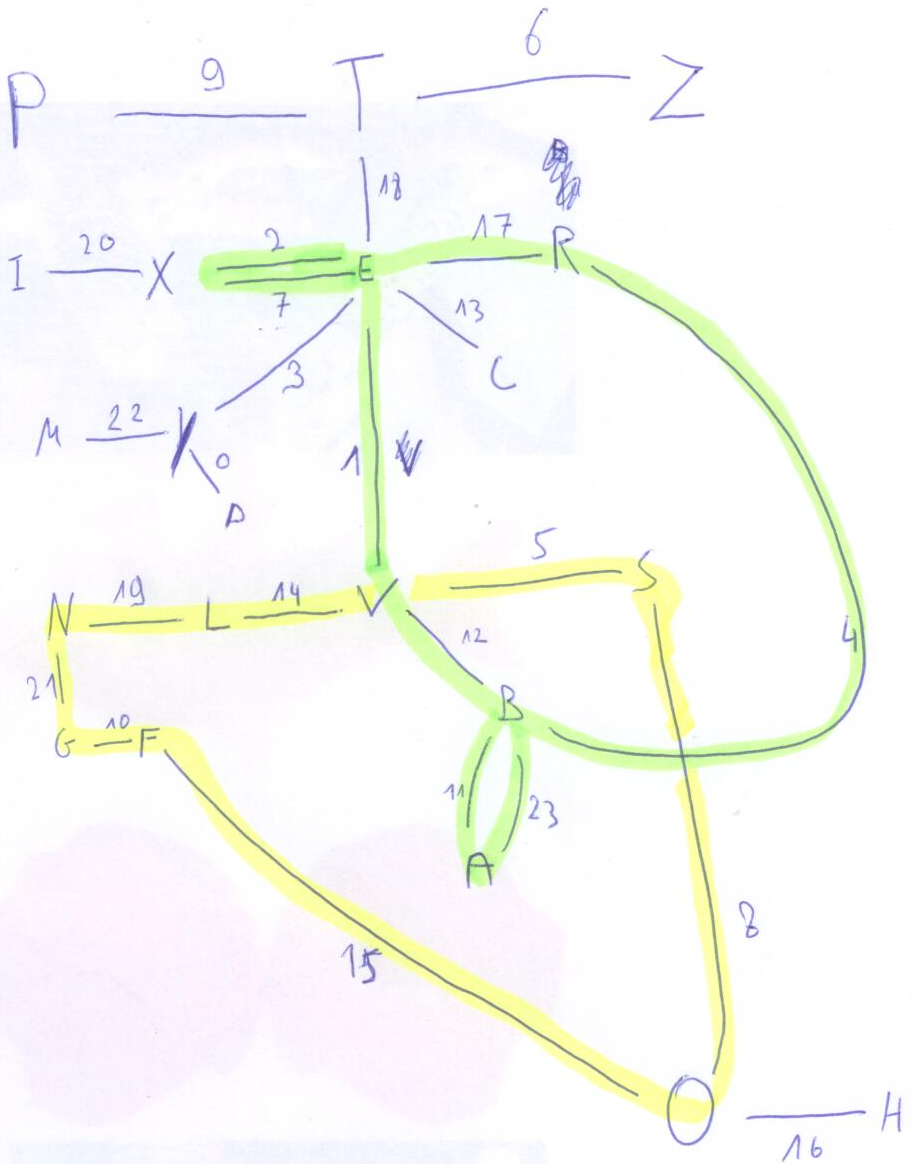
\includegraphics[width=0.5\linewidth]{Enigma}
		\caption[]{Enigma Graaf}
		\label{fig:enigma}
	\end{figure}

	Daaruit hebben we 4 onafhankelijke paden gevonden:
	\begin{enumerate}
		\item B $\rightarrow$ A $\rightarrow$ B
		\item E $\rightarrow$ X $\rightarrow$ E
		\item V $\rightarrow$ B $\rightarrow$ R $\rightarrow$ E $\rightarrow$ V
		\item V $\rightarrow$ S $\rightarrow$ O $\rightarrow$ F $\rightarrow$ G $\rightarrow$ N $\rightarrow$ L $\rightarrow$ V
	\end{enumerate}

	Er zijn dus fixpunten voor:
	\begin{enumerate}
		\item $\sigma \mathcal{E}_{k+11} \mathcal{E}_{k+23} \sigma$
		\item $\sigma \mathcal{E}_{k+2} \mathcal{E}_{k+7} \sigma$
		\item $\sigma \mathcal{E}_{k+5} \mathcal{E}_{k+8} \mathcal{E}_{k+15} \mathcal{E}_{k+10} \mathcal{E}_{k+21} \mathcal{E}_{k+19} \mathcal{E}_{k+14}\sigma$
		\item $\sigma \mathcal{E}_{k+12} \mathcal{E}_{k+4} \mathcal{E}_{k+17} \mathcal{E}_{k+1} \sigma$
	\end{enumerate}

	Deze hebben we dan manueel in onze kraker gestoken. Deze kraker probeert dan in alle mogelijke beginstanden een karakter te vinden die op zichzelf afbeelden door deze door de reeks van $\mathcal{E}_{k+i}$ te sturen. Omdat die nog altijd relatief veel mogelijkheden zullen zijn, gaan laten we daarna de ge\"{e}ncrypteerde tekst met die mogelijke beginstanden decoderen en kijken we of de tweede, derde en vierde letter dezelfde zijn. Die zullen gelijk zijn omdat deze letters gelijk zijn in de crib en het stekkerbord letters altijd op eenzelfde letter zal afbeelden. Dit dachten we dat het aantal mogelijkheden fel zou doen dalen en hebben we 's nachts op een server laten draaien.\\
	Daaruit bekwamen we nog altijd meer dan 300 mogelijkheden uit. Dit was te veel om met de hand na te kijken, dus lieten we er nog een check op uitvoeren.
	We laden de mogelijkheden in en gaan telkens een stekkerbord proberen te maken door te kijken naar de mapping van de crib tot de eerste letters van de gedecodeerde code. Daar mogen geen contradicties in zitten. Dit was jammer genoeg bij elke mogelijkheid wel het geval en uiteindelijk hadden we geen tijd meer om een andere oplossing te implementeren.
	\\
	Al de 327 mogelijkheden staan in de result.txt in de map Enigma. Het is telkens de setting van de Enigma machine gevolgd door de uitgeschreven code. Wat ons wel opviel was dat het vooral het 7de karakter (de vierde E) was die voor een fout zorgde in de mapping.
	
	
\end{document}